\documentclass[compileTAMUreport.tex]{subfiles}

\begin{document}
\chapter{Methodology}

For reference in this section, Figures \ref{fig:flowregime} and \ref{fig:boilingregime} give examples of the meaning of typical flow and boiling regimes, respectively.

%%%%%%%%%%%%%%%% begin FIGURE 2 %%%%%%%%%%%%%%%%%%%
\begin{figure}[H]
\begin{center}
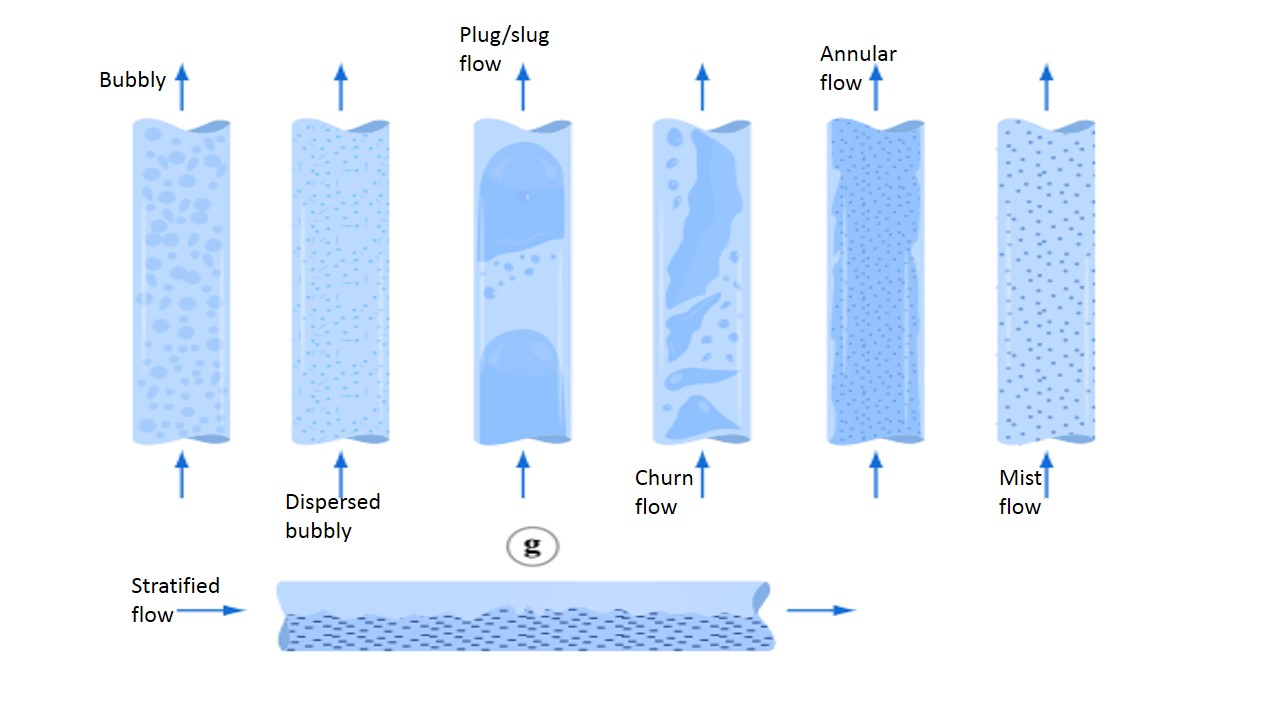
\includegraphics[width=0.75\textwidth]{./figure/flow_regime}
\end{center}
\caption{Flow Regime}
\label{fig:flowregime}
\end{figure}
%%%%%%%%%%%%%%%% end FIGURE %%%%%%%%%%%%%%%%%%

%%%%%%%%%%%%%%%% begin FIGURE 1 %%%%%%%%%%%%%%%%%%%
\begin{figure}[H]
\centering
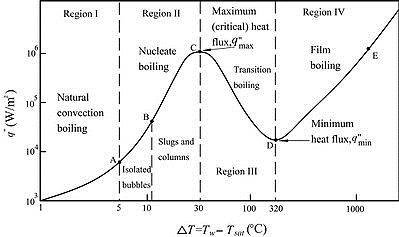
\includegraphics[width=0.5\textwidth]{./figure/400px-Boiling}
\caption{Boiling curve the caption of a single sentence does not have period at the end}
\label{fig:boilingregime}
\end{figure}
%%%%%%%%%%%%%%%% end FIGURE 1 %%%%%%%%%%%%%%%%%%%

\subsection{Assumptions}

It is necessary to clearly state our assumptions for the following analysis as many considerations have be approximated or considered on a theoretical basis since the actual effects are quite complex. 
In summary, our assumptions for the various sub-systems of our model require:
\begin{itemize} % System level
	\item Foams
		\begin{itemize}
			\item 	Error introduced by using Kelvin relation is acceptable versus computational effort for Weaire–Phelan structure. \cite{Kusner1996}
			\item The foam properties are constant through out.
			\item	Metal foam measurements are known to be inaccurate. 
			For a foam of 0.97 porosity ($\epsilon$), the Kelvin stucture with a spherical void to yield the given porosity can be optimized to an analytical geometry constructed of spheres and equilateral prisms that is equivalent to a metal foam.
			 
			[Bhattacharaya 		\& Mahajan 2002 AIAA] state that the limit of the equilateral triangle geometry extends to $\epsilon = 0.94$ before becoming a convex prism. 
			We take this as an error in our model that is reasonable to perform the calculations.\cite{Bhattacharya2002}
		\end{itemize}
		
\begin{figure}[H]
  \centering
    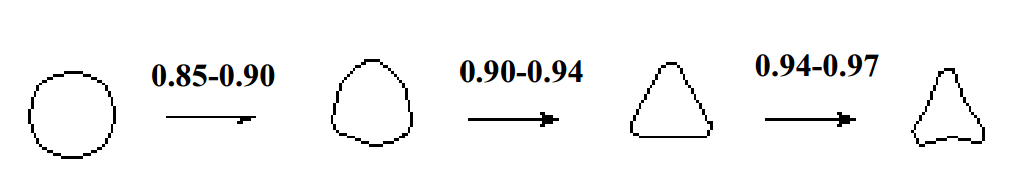
\includegraphics[width=0.5\textwidth]{./figure/porosityVariance}
  \caption{Ligament geometry variance with $\epsilon$}
\end{figure}

	\item Thermodynamics
		\begin{itemize}
			\item 	Real fluid properties: data is taken from Engineering Equation Solver (EES) and fitted using 2nd order equations. 
			\item 	For a pressure drop along the length of the tube/foam, the saturation temperature also changes with length of the pipe instantaneously in the next cell.
			\item The metal foam has constant properties.
			\item 	Stable thermal vaporization - a non-transient increase in vapor velocity with increasing mass fraction of vapor as a consequence of maintaining local saturation pressure and temperature in the vapor region.
		\item 	No fluid entrainment in vapor core for annular flow.
		\end{itemize}

\item Flows
	\begin{itemize}
		\item 	Only considering saturated, two phase flow.
		\item 	Inlet conditions are fully developed for the metal foam and non-metal foam cases
		\item 	Flow is turbulent on all length scales: tube and pore \cite{Incropera}
		\item 	Stable flow conditions. No transition schemes are modeled on any length scale.
		\item 	Only considering dispersed/bubbly and annular flows since the fluid is not subcooled before entering our analysis and the desired exit quality of the flow is 0.8 to remove any changes of exceeding the maximum heat flux at the wall. 
		Alternatively it could be said that we are not considering any form of dimensionalized intermediate flow regime (slug or churn). The transition occurs instantaneously in our model.
		\item	Two flow analysis methods are viable: homogeneous, where the properties are evaluated at the mixture quality, and separated where two regions are formed. These regions exist at the wall with pure fluid ($x=0$) and pure vapor at the core ($x=1$).
		Homogeneous is applicable in nucleate boiling regime for dispersed flows and separated is approximately applicable in annular flow since some dispersion does occur at nucleation sites within the liquid film at the wall.
	\item 	Superposition of pressure drops where the pressure drop from the foam is calculated using the Forschheimer-Darcy equation and the pressure drop from viscous effects at the tube wall is from the standard Darcy-Weisbach (
	Moody) method. See Calculations.
	\item Flow rate is for operation of a 500MW turbine. (1000 tubes with a 1 inch diameter (smallest diameter in this study).
	\end{itemize}

\item Heat Transfer
	\begin{itemize}
		\item 	Inlet temperature for the fluid is at saturation temperature
		\item 	Non-thermal equilibrium is assumed with the foam\cite{Xu2011}
		\item 	Steady state operating condition is assumed, thus convergence is possible for our method.
		\item 	Foam temperature is held at saturation temperature even though convection is modeled from the foam to the vapor. This allows for an approximate solution without considering superheating effects on the liquid film and the metal foam in the vapor region.
		\item 	No bubble confinement  (sub cooled boiling) required in our model since fluid is at \Tsat at entrance.
	\end{itemize}
\end{itemize}

\section{Analysis Methods}
The usage of metal foams in the boiler to enhance the heat transfer between the boiler and fluid  would effectively increase the rate at which the steam is produced thereby potentially reducing the length of the boiler.

The analysis of heat transfer in a metal foam can either be performed using a two energy equation volume averaged or a cell/lattice resolution method.
In the volume averaged method the effective surface area, relative density and effective heat transfer coefficient  are used to calculate the various heat transfer properties required to determine the desired results.

\cite{Du2010}
In the cell resolution method, the unit cell of a metal foam is modeled based on various assumption made about the formation of the cell. 
Lord Kelvin was the first to analyze the problem, and his model can be described as a tetrakaidecahedron, or terminated octahedron.
\cite{Kopanidis2010}
This is the model of choice for our study due to symmetry of the unit cell.

It should be noted that this is not the most accurate unit cell representation; the Weaire-Phelan (WP) structure has been proven to better solve the surface energy minimization problem of the interstitial gas bubble formation within metal foams.
The WP structure has an 8 cell group symmetry due to the use of 2 separate cell types, one of which is a irregular dodecahedron.
The basic structure was taken into consideration was to optimize the heat transfer rate and minimize the heat storage in the metal foam, this is basically done by increasing the surface area to volume ratio.
\cite{Kusner1996}

% This is the figure we need here.

%%%%%%%%%%%%%%%% begin FIGURE 1 %%%%%%%%%%%%%%%%%%%
\begin{figure}[H]
\begin{center}
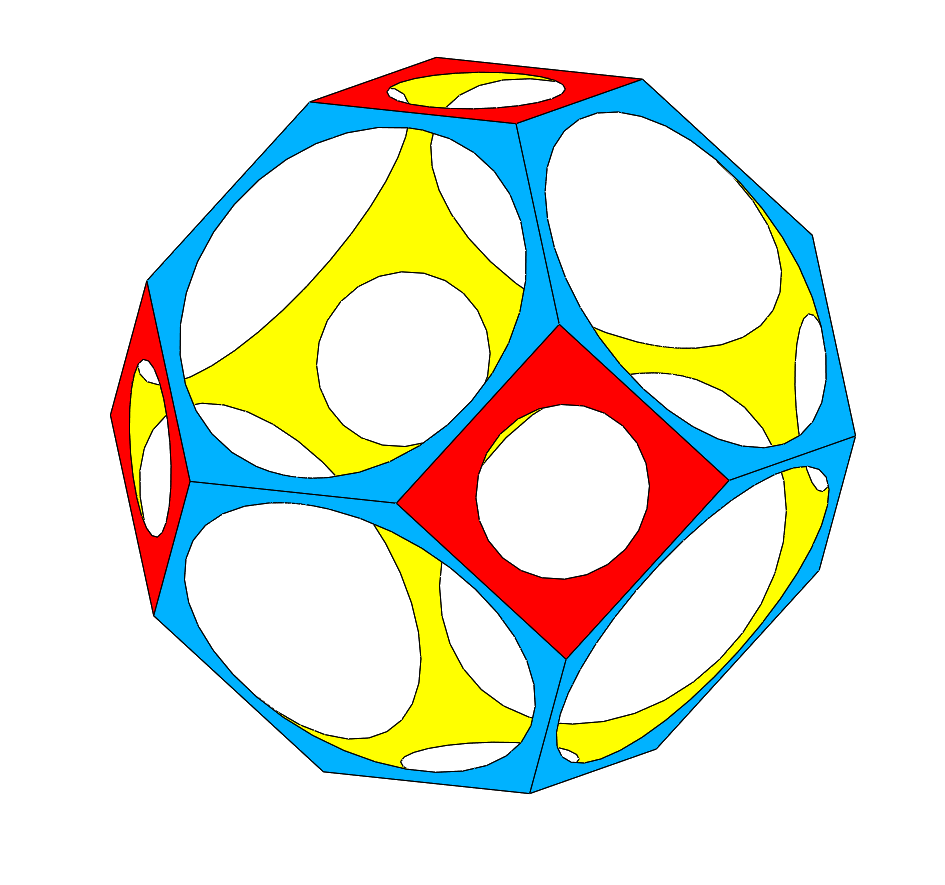
\includegraphics[width=0.35\textwidth]{./figure/TruncatedOctohedronSphereRemoved}
\end{center}
\caption{Terminated Octahedron Unit Cell also Known as a Kelvin Structure}
\label{fig:trucOctModel-UnitCell}
\end{figure}
%%%%%%%%%%%%%%%% end FIGURE %%%%%%%%%%%%%%%%%%

For our analytical model, we have taken a novel approach to modeling a fin network using the tetrakaidecahedron unit cell as the framework.
To our knowledge, no one has yet published any results using such a method. 
At the nodes, spheres will be placed and for the geometry of the ligaments, isosceles prismatic fins will connect to the spheres. 
A correction factor will be applied to take the sphere contact face as ``flat" to simplify the fin equations. 
Utilizing symmetry, of which the tetrakaidecahedron has symmetry along $90\degree, 120\degree,$ and $180\degree$, it will be determined which symmetry mode will be used to simplify this analytical study.


%% Go grab a good unit cell picture! 

%%%%%%%%%%%%%%%% begin FIGURE 2 %%%%%%%%%%%%%%%%%%%
\begin{figure}[H]
\begin{center}
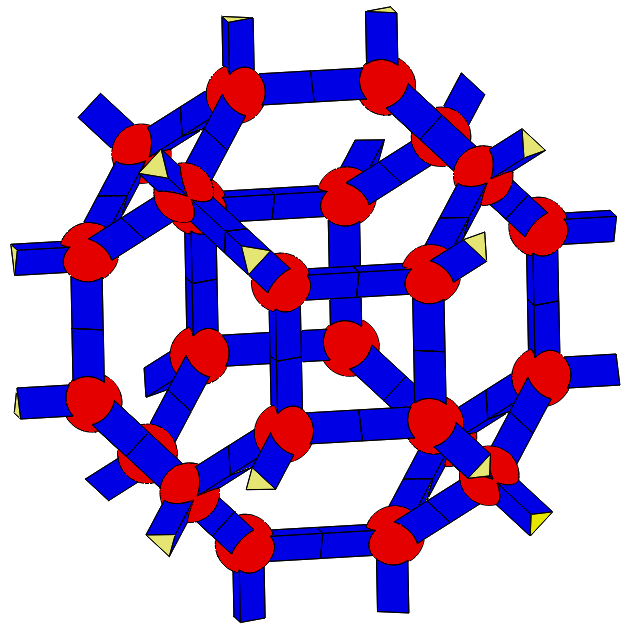
\includegraphics[width=0.35\textwidth]{./figure/AnalyticalUnitCell}
\end{center}
\caption{Analytical fin network with interstitial spheres at nodes}
\label{fig:flowregime}
\end{figure}
%%%%%%%%%%%%%%%% end FIGURE %%%%%%%%%%%%%%%%%%

The network of prisms and fins can be broken down by symmetric groupings along certain direction vectors, solved for nodal temperature using resistance analogy methods, and can be used to determine total convective heat transfer into the water. 
For our flow case, which is turbulent on both the tube and pore length scale, the following correlations for heat transfer coefficient can be used in a homogeneous regime.


\section{Calculations}

The Reynolds numbers used are

\begin{equation}
 Re_{\mathrm{pipe}} = \frac{\vec{v} D_{\mathrm{pipe}}}{\nu_f}, ~~~~~~ Re_{sph} = \frac{\vec{v} D_{sph}}{\nu_f} ~~~~ Re_{\mathrm{tri}} = \frac{\vec{v} a_{\mathrm{tri,edge}}}{\nu_f}
\end{equation}

For spheres in turbulent external flow the Nusslet correlation is\cite{Incropera}

\begin{equation}
Nu_{sph} = 2+ (0.4Re^{1/2} +0.06 Re^{2/3})Pr^{0.4} \left( \frac{\mu}{\mu_s} \right)
\end{equation}

which is valid for $3.5<Re<7.6\times 10^{4}$, $0.71<Pr<380$, and $1 < \mu / \mu_s 3.2$.

% Enter equation here... and CITE.
%which is valid for $< Pr  < $ and $ < Re <$. 
%As shown in Table \ref{tab:ReynoldsNumbers}, this relationship is valid for all flow conditions considered in this study.

For triangular prisms in turbulent external flow, very little data exists for $Nu_{tri}$. We suspect this is because of variance with angle of attack as it directly influences the flow field and subsequent advection. For this work, we use \ref{Chakrabarty2008} and averaged his values for all angle of attack. His Reynolds number was $2.6 \times 10^4$ which is beyond the Reynolds number for our triangular ligaments ($Re_{tri} ~ 150$). Additionally his experiment used air as the fluid at STP conditions. \cite{JAEGER2013}

\begin{equation}
Nu_{sph} = 455
\end{equation}

% Did we use the analogy or the "EXPERIMENTAL STUDY ON FLUID FLOW AND HEAT TRANSFER FROM A TRIANGULAR PRISM APPROACHING THE WALL OF A WIND TUNNEL (REYNOLDS NUMBER = 2.6×104) Dipes Chakrabarty, Ranajit Brahma Paper" ?  
% Enter equation here... and CITE.

The bound on heat flux into the tubes are given the the Zuber Kutateladze prediction for film boiling, such that

\begin{equation}
q_{max,z} = (\pi/24)\rho_g^{0.5} h_{fg} \sqrt[4]{g (\rho_{f} - \rho_{g}) \sigma}
\end{equation}

Although the Rohsenow prediction for the initiation of nucleate boiling gives a more accurate result for pipe flow, we will use Zuber's relation for the heat flux to initiate nucleate boiling since it is simpler and not as critical to our analysis.
\cite{Incropera}

\begin{equation}
q''_{min} = 0.009 \rho_g^{0.5} h_{fg} \left( \frac{g\sigma \left( \rho_f - \rho_g \right)}{(\rho_f + \rho_g)^2} \right)^0.25
\end{equation}

In order to evaluate the flux condition to get a temperature, we need the heat transfer coefficient. Although we do not yet have a relation for $h$ for the pipe with metal foam, we can use the standard Dottis-Boelter Nusslet correlation in Equation \ref{eq:Dottis-Boelter_Pipe} for pipe flow to calculate it for the pipe without metal foam. In order to correct, specifically for the assumed increase in heat transfer coefficient, we apply a scaling factor to the result. Empirical testing would validate this.

\begin{equation} \label{eq:Dottis-Boelter_Pipe}
Nu_{\mathrm{pipe}} = 0.023 Re^{(4/5)} Pr^{0.4}
\end{equation}
%
%For the condition specified in the EES code (see appendix) which had a saturation temperature of ___ we calculated the wall temperature to be ____ and the on set of nucleate boiling to occur at ___. 


Again, the basic aim of this project is to compare the effectiveness of a metal foam when used inside a boiler as well as to find the sensitivity of the heat transfer based on the various properties of a metal foam. Based on the previous work done in this field, the following properties have been taken into consideration for the simulation and analysis of the model

% Citations?

\begin{itemize}
	\item Independent
		\begin{enumerate}
			\item $\rho_{cell} : [10,40] \mathrm{PPI}$
			\item $\phi_{porosity}= 0.97$, maximized
			\item $\dot{m} = 882 \kilo\gram\per\second$, average
			\item $ q’’_(\mathrm{wall,max}) = 4.5 \kilo\watt\per\metre\squared$
			\item $ 0.025 < D_{\mathrm{pipe}} < .15 \metre$
			\item $ T_{in}=500 K ;P_{in} = 650 \kilo\pascal $
		\end{enumerate}
	\item Dependent
		\begin{enumerate}
			\item $100 < Re_{d_p} < 2.5 \times 3$
			\item $K_{permeability}= f(\Delta P)$
		\end{enumerate}
\end{itemize}

\end{document}